% \documentclass{article}
\documentclass[fleqn]{article} 
\usepackage{amsmath}
\usepackage{enumitem}
\usepackage{import}
\subimport*{./}{macro}

\setlength\parindent{20px}
\setlength{\mathindent}{20pt}

\begin{document}
\title{Homework \#1}
\author{Aaron Chen / aaronyc}
\date{}
\maketitle

% ------ setting ------

\subsection*{A1.}

\begin{enumerate}[label=(\alph*)]
\item
\begin{itemize}
\item Bias: The distance between the model's average prediction and the ground-truth model.
\item Variance: How much the model changes when it is trained on different training data.
\item Bias-variance tradeoff: As a model gets closer to the ground truth, it often becomes easier to disrupt by the particular training data.
\end{itemize}

\item
With higher model complexity, the model can fit the training data more closely, so bias typically decreases, but variance typically increases.
With lower model complexity, the model is less flexible, so bias typically increases, but variance typically decreases.

\item
False.

Using fewer features does not always improve generalization.  \\
It may reduce variance, but it can also remove useful information and increase bias.

\item
False.

Hyperparameters should be tuned on a validation set, not the test set.  \\
For example, we can use k-fold cross-validation by splitting the training data into training and validation folds, trying different hyperparameter values, and choosing the one with the best average validation performance. \\
The test set should only be used once at the end to estimate final generalization performance.

\item
False.

Training error is usually an underestimate of the true error because the model was fit on the training set. \\
The true error is better estimated using unseen validation or test data.

\end{enumerate}

% ---------------------

\subsection*{A2.}

\begin{enumerate}[label=(\alph*)]
\item
\[
X_1, X_2, \dots, X_n \overset{\text{iid}}{\sim} \operatorname{Poisson}(\lambda)
\]

\[
P(X = x) = \frac{e^{-\lambda}\lambda^x}{x!}
\]

\begin{align*}
L(\lambda)
&= \prod_{i=1}^{n} P(X_i = x_i) \\
&= \prod_{i=1}^{n} \frac{e^{-\lambda}\lambda^{x_i}}{x_i!} \\
&= \left(\prod_{i=1}^{n} e^{-\lambda}\right)
   \left(\prod_{i=1}^{n} \lambda^{x_i}\right)
   \left(\prod_{i=1}^{n} \frac{1}{x_i!}\right) \\
&= \frac{e^{-n\lambda}\lambda^{\sum_{i=1}^{n}x_i}}{\prod_{i=1}^{n}x_i!}
\end{align*}

\begin{align*}
\ell(\lambda)
&= \log L(\lambda) \\
&= \log\left(\frac{e^{-n\lambda}\lambda^{\sum_{i=1}^{n}x_i}}{\prod_{i=1}^{n}x_i!}\right) \\
&= \log\left(e^{-n\lambda}\right)
   + \log\left(\lambda^{\sum_{i=1}^{n}x_i}\right)
   - \log\left(\prod_{i=1}^{n}x_i!\right) \\
&= -n\lambda + \left(\sum_{i=1}^{n}x_i\right)\log \lambda
   - \sum_{i=1}^{n}\log(x_i!)
\end{align*}

\begin{align*}
\frac{\dd}{\dd \lambda}\ell(\lambda)
&= -n + \frac{\sum_{i=1}^{n}x_i}{\lambda}
\end{align*}

\begin{align*}
-n + \frac{\sum_{i=1}^{n}x_i}{\lambda} &= 0 \\
\frac{\sum_{i=1}^{n}x_i}{\lambda} &= n \\
\sum_{i=1}^{n}x_i &= n\lambda
\end{align*}

\[
\hat{\lambda}_{\text{MLE}} = \frac{1}{n}\sum_{i=1}^{n}x_i
\]

\item
\[
\hat{\lambda}_{MLE}
= \frac{2+4+6+0+1}{5}
= \frac{13}{5}
= 2.6
\]

\begin{align*}
\mathrm{Poi}(X=6)
&= e^{-2.6}\frac{2.6^6}{6!} \\
&\approx 0.0319
\end{align*}

\item
\[
\hat{\lambda}_{MLE}
= \frac{13+8}{5+1}
= \frac{21}{6}
= 3.5
\]

\begin{align*}
\mathrm{Poi}(X=6)
&= e^{-3.5}\frac{3.5^6}{6!} \\
&\approx 0.0771
\end{align*}
\end{enumerate}

% ---------------------

\subsection*{A3.}

Increasing regularization makes the learned polynomial smoother and less sensitive to individual training points.
Compared with $\lambda = 0$, the model with $\lambda = 1$ has lower variance and is less likely to overfit, but it may introduce more bias.

\begin{center}
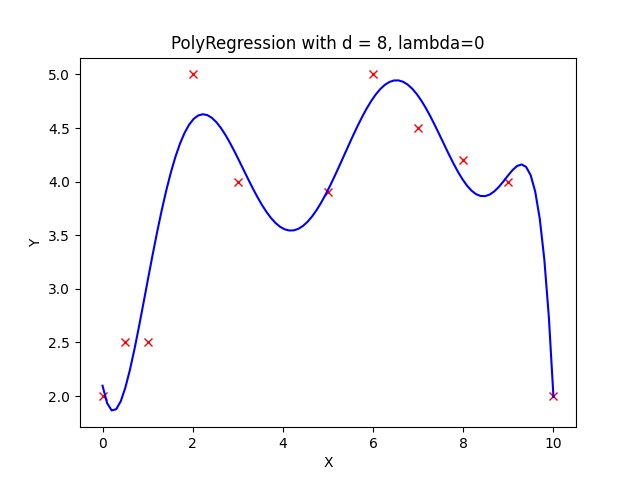
\includegraphics[width=0.8\textwidth]{hw1-A/homeworks/poly_regression/hw1_A_Figure_1_lambda_0.png}
\end{center}

\begin{center}
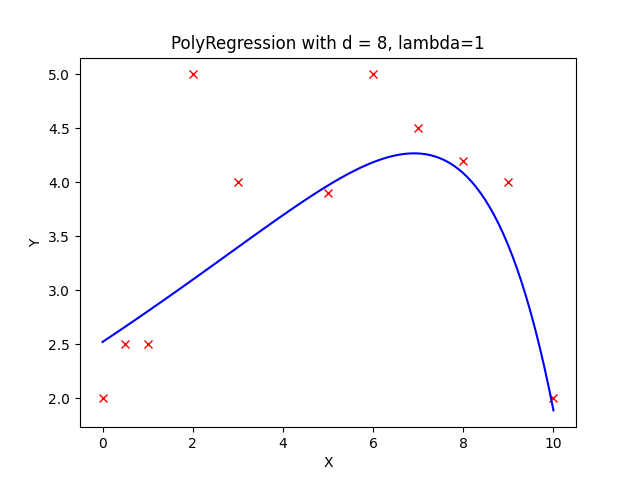
\includegraphics[width=0.8\textwidth]{hw1-A/homeworks/poly_regression/hw1_A_Figure_1_lambda_1.png}
\end{center}

% ---------------------

\subsection*{A4.}

\begin{center}
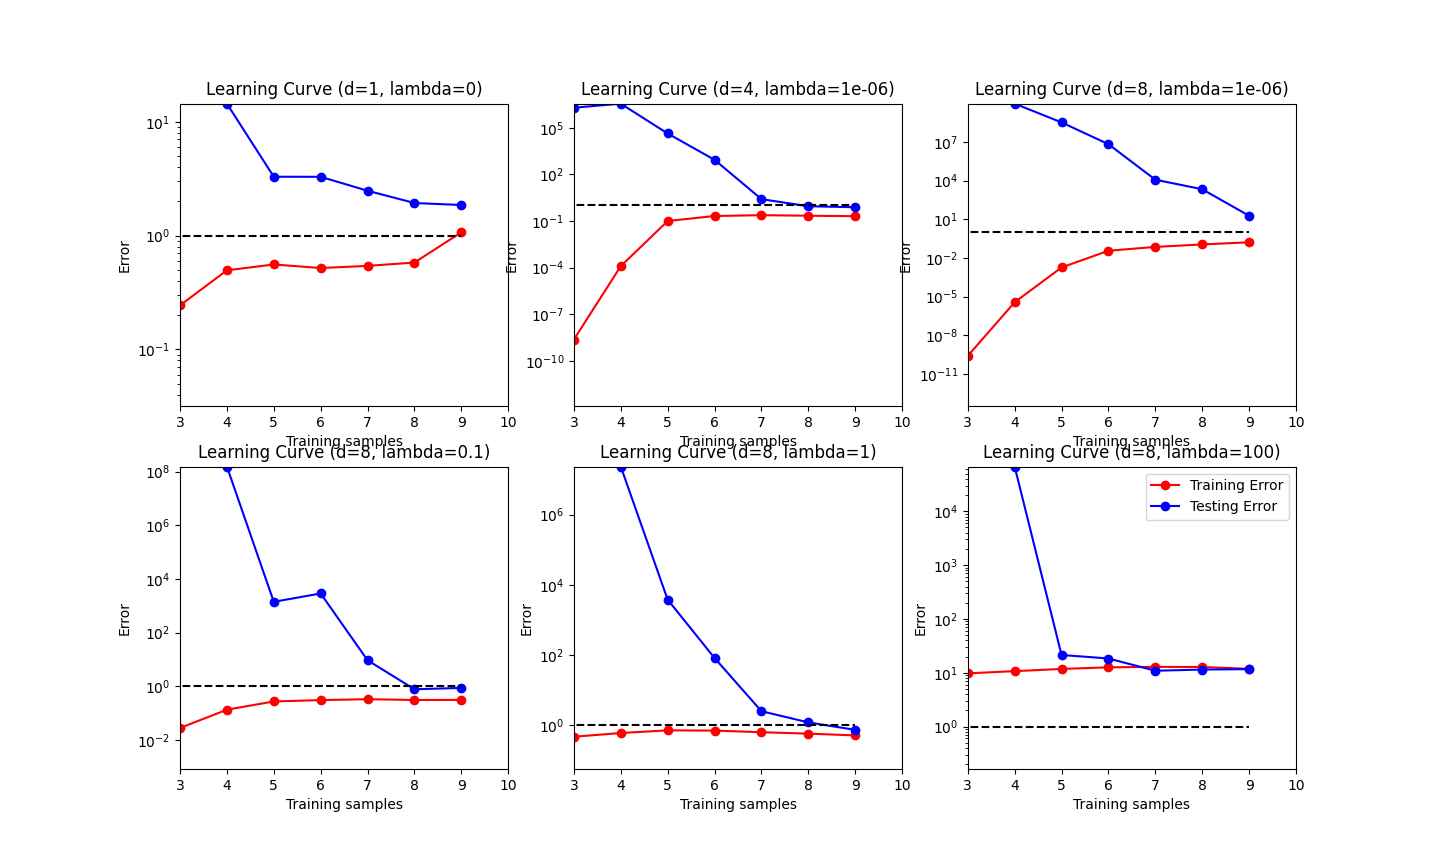
\includegraphics[width=\textwidth]{hw1-A/homeworks/poly_regression/hw1_A_Figure_2.png}
\end{center}

% ---------------------

\subsection*{A5.}

\begin{enumerate}[label=(\alph*)]
\item
\[
\widehat{W}
= \argmin_{W \in \R^{d \times k}}
\sum_{i=1}^{n} \|W^\top x_i - y_i\|_2^2 + \lambda \|W\|_F^2
\]

\[
X =
\begin{bmatrix}
x_1^\top \\
x_2^\top \\
\vdots \\
x_n^\top
\end{bmatrix}
\in \R^{n \times d},
\qquad
Y =
\begin{bmatrix}
y_1^\top \\
y_2^\top \\
\vdots \\
y_n^\top
\end{bmatrix}
\in \R^{n \times k}
\]

\begin{align*}
J(W)
&= \|XW - Y\|_F^2 + \lambda\|W\|_F^2 \\
&= \sum_{j=1}^{k}\left(\|Xw_j - Ye_j\|_2^2 + \lambda\|w_j\|_2^2\right)
\end{align*}

\[
J_j(w_j) = \|Xw_j - Ye_j\|_2^2 + \lambda\|w_j\|_2^2
\]

\begin{align*}
J_j(w_j)
&= (Xw_j - Ye_j)^\top(Xw_j - Ye_j) + \lambda w_j^\top w_j
\end{align*}

\begin{align*}
\nabla_{w_j} J_j(w_j)
&= 2X^\top(Xw_j - Ye_j) + 2\lambda w_j \\
&= 2X^\top Xw_j - 2X^\top Ye_j + 2\lambda w_j
\end{align*}

\begin{align*}
2X^\top Xw_j - 2X^\top Ye_j + 2\lambda w_j &= 0 \\
(X^\top X + \lambda I)w_j &= X^\top Ye_j \\
\widehat{w}_j &= (X^\top X + \lambda I)^{-1}X^\top Ye_j
\end{align*}

\begin{align*}
\widehat{W}
&= \begin{bmatrix}
\widehat{w}_1 & \widehat{w}_2 & \cdots & \widehat{w}_k
\end{bmatrix} \\
&= (X^\top X + \lambda I)^{-1}X^\top
\begin{bmatrix}
Ye_1 & Ye_2 & \cdots & Ye_k
\end{bmatrix} \\
&= (X^\top X + \lambda I)^{-1}X^\top Y
\end{align*}

\item

\[
\widehat{\epsilon}_{\textrm{train}} = 14.805\%
\]

\[
\widehat{\epsilon}_{\textrm{test}} = 14.66\%
\]
\end{enumerate}

% ---------------------

% ------ setting ------

\end{document}
